%% Copernicus Publications Manuscript Preparation Template for LaTeX Submissions
%% ---------------------------------
%% This template should be used for copernicus.cls
%% The class file and some style files are bundled in the Copernicus Latex Package, which can be downloaded from the different journal webpages.
%% For further assistance please contact Copernicus Publications at: production@copernicus.org
%% https://publications.copernicus.org/for_authors/manuscript_preparation.html


%% Please use the following documentclass and journal abbreviations for preprints and final revised papers.

%% 2-column papers and preprints
\documentclass[journal abbreviation, manuscript]{copernicus}


%% Journal abbreviations (please use the same for preprints and final revised papers)


% Advances in Geosciences (adgeo)
% Advances in Radio Science (ars)
% Advances in Science and Research (asr)
% Advances in Statistical Climatology, Meteorology and Oceanography (ascmo)
% Annales Geophysicae (angeo)
% Archives Animal Breeding (aab)
% Atmospheric Chemistry and Physics (acp)
% Atmospheric Measurement Techniques (amt)
% Biogeosciences (bg)
% Climate of the Past (cp)
% DEUQUA Special Publications (deuquasp)
% Drinking Water Engineering and Science (dwes)
% Earth Surface Dynamics (esurf)
% Earth System Dynamics (esd)
% Earth System Science Data (essd)
% E&G Quaternary Science Journal (egqsj)
% EGUsphere (egusphere) | This is only for EGUsphere preprints submitted without relation to an EGU journal.
% European Journal of Mineralogy (ejm)
% Fossil Record (fr)
% Geochronology (gchron)
% Geographica Helvetica (gh)
% Geoscience Communication (gc)
% Geoscientific Instrumentation, Methods and Data Systems (gi)
% Geoscientific Model Development (gmd)
% History of Geo- and Space Sciences (hgss)
% Hydrology and Earth System Sciences (hess)
% Journal of Bone and Joint Infection (jbji)
% Journal of Micropalaeontology (jm)
% Journal of Sensors and Sensor Systems (jsss)
% Magnetic Resonance (mr)
% Mechanical Sciences (ms)
% Natural Hazards and Earth System Sciences (nhess)
% Nonlinear Processes in Geophysics (npg)
% Ocean Science (os)
% Polarforschung - Journal of the German Society for Polar Research (polf)
% Primate Biology (pb)
% Proceedings of the International Association of Hydrological Sciences (piahs)
% Safety of Nuclear Waste Disposal (sand)
% Scientific Drilling (sd)
% SOIL (soil)
% Solid Earth (se)
% The Cryosphere (tc)
% Weather and Climate Dynamics (wcd)
% Web Ecology (we)
% Wind Energy Science (wes)


%% \usepackage commands included in the copernicus.cls:
%\usepackage[german, english]{babel}
%\usepackage{tabularx}
%\usepackage{cancel}
%\usepackage{multirow}
%\usepackage{supertabular}
%\usepackage{algorithmic}
%\usepackage{algorithm}
%\usepackage{amsthm}
%\usepackage{float}
%\usepackage{subfig}
%\usepackage{rotating}
\usepackage{bm}
\usepackage[normalem]{ulem}
\theoremstyle{definition}
\newtheorem{definition}{Definition}[section]
\newtheorem{observation}{Observation}[section]

\newcommand{\om}[1]{{\color{red} objection $^{#1}$}: }
\newcommand{\cm}[1]{{\color{green} statement $^{#1}$} }
\newcommand{\oc}[2]{{\color{red} #1  $^{#2}$}}
\newcommand{\cc}[2]{{\color{green} #1  $^{#2}$}}
\newcommand{\X}{\mathbf{X}}
\newcommand{\I}{\mathbf{I}}
\renewcommand{\O}{\mathbf{O}}
\newcommand{\RT}{\mathbf{RT}}
\newcommand{\bv}{\bm{\beta}}
\newcommand{\figref}[1]{Fig. \ref{#1}}
\DeclareMathOperator{\sign}{sign}

%\graphicspath{{../figures/}}
\begin{document}

\title{Applications and limits of the quasi steady state approximations for nonautonomous compartmental systems}


% \Author[affil]{given_name}{surname}

\Author[]{Markus}{Müller}
\Author[]{Konstiantin}{Viatkin}
%\Author[]{Yiqi}{Luo}

\affil[]{ADDRESS}
\affil[]{ADDRESS}

%% The [] brackets identify the author with the corresponding affiliation. 1, 2, 3, etc. should be inserted.

%% If an author is deceased, please mark the respective author name(s) with a dagger, e.g. "\Author[2,$\dag$]{Anton}{Smith}", and add a further "\affil[$\dag$]{deceased, 1 July 2019}".

%% If authors contributed equally, please mark the respective author names with an asterisk, e.g. "\Author[2,*]{Anton}{Smith}" and "\Author[3,*]{Bradley}{Miller}" and add a further affiliation: "\affil[*]{These authors contributed equally to this work.}".


\correspondence{Markus Müler(mm2796@cornell.edu)}

\runningtitle{Applications and limits of the quasi steady state approximations for nonautonomous compartmental systems}

\runningauthor{Markus Müller}





\received{}
\pubdiscuss{} %% only important for two-stage journals
\revised{}
\accepted{}
\published{}

%% These dates will be inserted by Copernicus Publications during the typesetting process.


\firstpage{1}

\maketitle



\begin{abstract}
%This  paper has been prompted by a series of claims in the original work \citep{Luo2017Biogeosciences} .
Quasi steady state descriptions are used as approximations for transient systems for many reasons out of necessity.
It is important to know in which situations which of their assumed properties become misleading. 
%This work investigates those claims in the broader mathematical context 
%and attempts to illustrate some of the central concepts, their limits and how they should be interpreted. 

An important example is 'Carbon Storage Capacity' $\X_c$. The original publication describes the geometric relationship between $\X_p=\X-\X_c$ and the derivative $\dot{\X}$ of $\X$ with respect to time and infers that $\X_c$ is an 'attractor'.  
We formalize this relationship as far as we can prove it.
%which is that both vectors stay in the same orthant if the components of the poolwise difference between $\X_c - \X$ have all the same sign, and therefore the solution $\X$ never ``pulls away'' from $\X_c$.
As a result it becomes aparrent that these properties are indeed not sufficient to draw the conclusion that $\X_c$ 
attracts the solution $\X$ of the nonautonomous system. We provide a counterexample.

We also show that although $\X_c(t)$ is not an attractor for the actual carbon content it is a stable fix point for a related 'frozen' autonomous system. 

This frozen system also provides the proper context in which  variables related to $\X_c$ like ``chasing time'', ``residence time'' $\RT$ and ``carbon storage potential'' $\X_p$ can be interpretated.

We also provide a scalar surrogate system for the overall mass $x=\sum_{i=1,\dots,n} X_i$ of the system for which some simpler statemetns can be shown which are hard to generalize to the vector $\X_c$.


Complementary to the original work, which starts with analysis of 250 published papers about Carbon cycle models we will approach the traceability framework from the mathematical perspective of general compartmental models and discuss the additionally factorizability assumptions with respect to the models they exclude.
Regarding the ``environmental scalars'' $\xi$ and base line rates $k$  we show that they are not unambiguously defined by the model but a choice in it's formulation.
Only the product is a diagnostic model property.


In the application of the traceability analysis {\color{red} cite Lifen, Xia ...} $\X_c$ appears as a proxy for $\X$. Actually in fact it's temporal mean $\bar{\X_c}$ is used. 
We show that the accuracy of this approximation depends very much on the length of the time interval over which the mean is taken.

\end{abstract}


\copyrightstatement{TEXT} %% This section is optional and can be used for copyright transfers.


\introduction  %% \introduction[modified heading if necessary]
We first present the definitions of the ``Transient Tractability Analysis'' 
from the viewpoint of the theory of compartmental systems in order to show which parts are generally applicable and which rely on specific assumptions. 
This approach is complementary to the original presentation insofar as it is not restricted to actually \emph{published} but to mathematically {\it possible} models.  
The first of the diagnostic variables that we will look at more closely is the so called ``carbon storage capacity'' $\X_c$, the motivation behind it's definition, provable mathematical properties and interpretation.
Later we will look at the more specific ``environmental scalars'' $\xi$.


\subsection{Traceability analysis}
The traceability analysis defines several diagnostic variables using as much algebraic structure of the mass balance equation as is available.
Not all diagnostic variables are possible for all compartmental models. 

We chose here to introduce the diagnostic variables not all at once but rather in the order of decreasing generality.

The first diagnostic variables are available for all compartmental models and need no additional assumptions. 
In the later parts of this section we then assume to be able to identify more and more specific terms in the mass balance equation and use those to derive and trace ever more specific diagnostics.
Thus the very first part is valid for all models but how many of the later parts are applicable to a specific model  depends on how much we know about it.  

\subsubsection{Derivation of the matrix representation} 
We adapt the derivation originally found in \citep{Jacquez1972} in order to refer to it's implication for the generality of the formulation used in \citep{Luo2017Biogeosciences}.
Mathematically Compartmental Models are most economically described as graphs, where the set of compartments $\mathcal{P}$ and the set of non-negative fluxes $\mathcal{F}$ form the the nodes and edges respectively.  
Choosing numbers as indices we can enumerate  the set of pools $\mathcal{P}=\{p_0,\dots,p_n\}$ where $p_0$ is the outside world and write:
\begin{align*}
%\X  &=(x_1,\dots x_n)^T
%\\
\mathcal{F} &=
\{
I_{0 \rightarrow j} > 0
\text{ for } j \in \{1,\dots ,n\}
\}  
\\
&
\cup
\{
F_{i \rightarrow j} > 0
\text{ for } i \in \{1,\dots ,n\} 
\text{ and } j \in \{1,\dots ,n\} j\ne i
\}
\text{ with }
F_{i \rightarrow j}=0 \text{ for }  x_{i} = 0 
\}
\\
&
\cup
\{
F_{i \rightarrow 0} 
\text{ for } i \in \{1,\dots ,n\} 
\text{ with }
F_{i \rightarrow 0}=0 \text{ for }  x_{i} = 0 
\}
\end{align*}
\eqref{massbalance} back into a set of equations for single fluxes from which
it was originally derived \citep{Jacquez1972} and for which massbalance is guaranteed by definition.
where $x_i$ is the content of pool $p_i$,
$ 
I_{0 \rightarrow j} 
$
are influxes from the outside into the system 
$
F_{i \rightarrow j} 
$
are fluxes between pools 
and 
$
F_{i \rightarrow 0} 
$
are fluxes out of the system.
In general all fluxes can depend on the $x_i$  and time $t$ (trough environmental factors like  Temperature $T(t)$ and moisture $W(t)$.

The influxes don't have to depend on the $x_i$  but internal and out fluxes must at least depend on their source pool content to guarantee the 
condition that there is no outflux from an empty pool. 
% $
% F_{i \rightarrow * }=0 \text{ for }  \X_{i} = 0 
% $.
% Where we used the $*$ to indicate either another pool or the outside.
For every pool we have a mass balance equation.
\begin{align}
  \frac{d}{d t} x_i 
    &= 
    \sum_{j\ne i} (-F_{i\rightarrow j}+F_{j\rightarrow j}) + I_{0 \rightarrow i} - F_{i \rightarrow 0} \quad \forall i \in \{1,\dots n\}
    \\
    &= - \underbrace{
      \left(
      r_{i \rightarrow } 
      + 
      \sum_{j \ne i} r_{j,i}
      \right)
      }_{=m_{i,i}}
      x_i
      +
      \sum_{j \ne i} \underbrace{r_{i,j}}_{- m_{i,j}} x_j
      +
      F_{\rightarrow i}
    \\
    &= 
      -\sum_{j} m_{i,j} x_j + I_{\rightarrow i}
    \\
  \frac{d}{d t} \X &= \I(\X,t) - M(\X,t) \X \label{massbalance_0}
\end{align}
where we wrote $F_{i \rightarrow j} = r_{j,i} x_i \text{ for } i \in \{1, \dots n\} , j \in \{ 0, 1,\dots ,n\} \text{ and } j \ne i $ under the smoothness condition that $F \in \mathcal C^1$ \citep{Jacquez1972} 
$\X=(x_1,\dots x_n)^T$ for the ordered tuple of all pool contents, and $\I=(I_{\rightarrow 1},\dots I_{\rightarrow n})^T$ for the ordered tuple of all influxes.
$-M$ is called the Compartmental matrix.

\subsubsection{Matrix decomposition} 
Together with a start-value $\X_0$ \eqref{massbalance_0}  constitutes an "initial value problem" (ivp) which can be solved numerically by moving step by step forward in time.

%Note: 
%
%It is mathematical standard notation to use $X$ in the *formulation* of the ivp (representing the momentary value) althoug *after we have solved it* the solution is expressed as function of time $X(t)$. This avoids confusion since everything appering with arguments is recognizable as explicitly calculable *before* we have solved the ivp.

The system is "nonautonomous" (if either of $\I$ or $M$ depend on time $t$) and "nonlinear" if either $M$ dependents on $X$ or $\I$ cannot be written in the form $\I(\X,t)=I(t)\X$.

If $m_{i,i}(\X,t) \ne 0$ it is possible to factorize $M(X,t)$ into a product $M=A(\X,t) K(\X,t)$ where $K$ is a  diagonal matrix and the matrix $A$ has only ones on it's main diagonal. 

It is always possible to write $\I(\X,t)=\bv(\X,t)u(\X,t)$ where the scalar $u=\sum_{k=1\dots n} \I_k$  and the dimensionless vector $\bv = \I/u$ where $\sum_{k=1\dots n} \beta_k =1$
Using these terms  we arrive at 
\begin{align*}
\frac{d \X}{d t}&=B(\X,t) u(\X,t) - A(\X,t) K(\X,t) \X   
\end{align*}
\newcommand{\kiixt}{
      \left(
      r_{i \rightarrow } (\X,t)
      + 
      \sum_{l \ne i} r_{l,i} (\X,t)
      \right)
}
with:
\begin{align}
  k_{i,i}(\X,t) &=\kiixt \nonumber
  \\
  a_{j,i}(\X,t)  
  &=\frac{r_{j,i}}{k_{i,i}}=
  \left\{
  \begin{matrix}
    =\frac{
    r_{i,j} (\X,t)
  }{
    \kiixt
  } \text{ for } j \ne i
  \\
  1 \text{ for } j=i
  \end{matrix}
  \right.
  \label{aij}
\end{align}
The $k_{i,i}$ can be interpreted as the rate of the total flux out of pool $i$. The elements of column $i$ of $A$ describe then which fractions of this total outflux is transferred to pool $j$. 
Note that at this point the $k_i$ and $a_{i,j}$ are not assumed to be constant but possibly functions of time and $\X$. Therefore writing $M(\X,t) = A(\X,t) K(\X,t)$ is not a big assumption.
but note that inferring $A$ and $K$ from a given $M$ requires $m_{i,i} \ne 0$

\subsubsection{Assumption of Linearity}
If we assume the model to be linear and nonautonomous the dependency on $X$ vanishes and we have
\begin{align*}
\end{align*}
\begin{align}
\frac{d \X}{d t}
  &=\I(t) - M(t) \X \label{massbalance_linear}
  \\
  &= \bv(t)u(t) - A(t) K(t) \X \nonumber .
\end{align} 
This excludes certain models e.g. the interactions between chemical species in one compartmental model. 
Imagine that some of the pools contain Nitrogen and others Carbon .
It is likely that some fluxes out of carbon pools are controlled by the
available Nitrogen.  
Imagine a compartmental system where the startvector
consist of Carbon and Nitrogen pool contents: $\X=(c_1,c_2,\dots,
n_1,n_2,\dots )^T$, then a flux between carbon pools $a$ and $b$ that
depends of the content of nitrogen pool $c$ depends on (a part of) the
statevector, which makes it nonlinear.
\begin{align*}
F_{a \rightarrow b} (\X,t)  &= r_{c_i \rightarrow *}(n_c,t) \X_a \\
                            &= r_{c_i \rightarrow *}(\X,t) \X_a
\end{align*}


\subsubsection{Assumption of Factorizability, substrate centered versus flux centered description}
For many published models the nonautonomous part  can be further localized into a diagonal matrix $\xi(t)$ so that we can achieve constant $A$ and $K$. It is important to realize two points here:
\begin{enumerate}
\item \label{substrate_xi}
  This is not possible for all compartmental matrices.
\item  \label{define_xi}
  In the cases where it is possible it does not uniquely define $\xi$.
\end{enumerate}

We can discuss (\ref{substrate_xi}) from a mathematical and a modeling viewpoint:
\newcommand{\kiit}{
      \left(
      r_{i \rightarrow } (t)
      + 
      \sum_{l \ne i} r_{l,i} (t)
      \right)
}
The linear version of \eqref{aij} is: 
\begin{align}
  k_{i,i}(t) &=\kiit \nonumber
  \\
  a_{j,i}(t) &=\left\{
  \begin{matrix}
  \frac{
    r_{j,i} (t)
  }{
    \kiit
  } \text{ for } j \ne i
  \\
  1 \text{ for } j=i
  \end{matrix}
  \right.
  \label{aij}
\end{align}

From this representation it is clear that the $a_{i,j}$ are only constant if all rates $r_{j,i} \text{ for } j \in \{0,\dots ,n \}$ contain the \emph{same} time dependent factor $\xi(t)$ , which makes the existence of constant $A$ and $K$ 
an assumption.
From a modeling point of view the $\xi_{i,i}$ can be seen as a ``substrate'' dependent rate modifier since it affects everything that leaves the same pool in the same way, whereas $r_{i,*}(t)$ is specific to a single flux an so could be different for different ``processes'' even if they use the same substrate.


In order to discuss (\ref{define_xi}) we note that the assumption that we can write 
$M=A \xi K$ implies that we can also write it as $M=A \tilde{\xi} \tilde{K}$
where $\tilde{\xi}=d\xi$ , $\tilde{K}=d^{-1} K$ for any diagonal matrix $d$.
This implies that without further assumptions it is not possible to compute $\xi$
for a given model without a gauge condition like $\xi(T_0, W_0)=1$ for a some
specific temperature $T_0$ and moisture $W_0$, which in turn implies that the {\it baseline residence time } $(A K)^{-1}$
is only defined up to the above mentioned diagonal matrix $d$.
This fact becomes very important when certain properties of models are attributed to either $\xi$ or the {\it baseline residence time}.
Any sensible attribution of this kind has to be shown to be robust to changes of $d$.
\ref{xi_examples}

\subsubsection{Assumption of factorizability of $\xi$} 
In some cases we can resolve $\xi$ further.
$$
\frac{d X}{d t} = B(t)u(t) - A \xi_{temp}(t) \xi_{mois}(t) K X  
$$







\subsection{Definition of diagnostic variables}

\subsubsection{Storage capacity $X_c$ and storage potential $X_p$}
These variables can be defined for any compartmental system and do not require either linearity nor factorizability. 
We can rearrange \eqref{massbalance_0} and give names to the two summands. 
$$
X = M^{-1}(\X,t) \left(\I(\X,t)- \frac{d \X}{d t} \right) \\ 
  = \underbrace{M^{-1}(\X,t)\I(\X,t)}_{\X_c} - \underbrace{M^{-1}(\X,t) \frac{d \X}{d t} }_{\X_p} \\
  = \X_c - \X_p
$$
Note:
This is not to be read as a recipe to compute $\X$.
The equation becomes a bit clearer if we adapt the nomenclature to express that we *have solved the ivp* and know its solution $\X(t)$  
and therefore also  the derivative $\frac{d \X}{d t}=I(\X(t),t) - M(\X(t),t) \X(t) =\dot{\X}(t)$ 
By substituting the solution $\X(t)$ we get the recipes to compute:
$$
\dot{\X}(t) = \I(\X(t),t) - M(\X(t),t) \X \\
\X_c(t) = M^{-1}(\X(t),t)\I(\X,t) \\ 
\X_p(t) = \X(t)-\X_c(t) \\ 
$$
we see that all the ingredients become explicit functions of time.   
\footnote{
  Since all values are taken at the same time $t$ we can drop the time dependence
  in the notation and write an equation we can use in the iterator.
  $$
  \dot{\X} = \I - M \X \\
  \X_c = \X + \X_p \\ 
  \X_p = M^{-1}I  \\ 
  $$
}
\subsubsection{Residence Time $\RT$}
The influx $\I$ can always be written as $\I=\bv u$ .
Assuming that the pool contents (the components of $\X$)  have dimension $mass$ we can infer from \eqref{massbalance_0}) that the components of $M$ have dimension $\frac{1}{time}$.
The components of the (inverse) matrix $M^{-1}$ have therefore dimension $time$. Accordingly the product $\RT= M^{-1} \bv$ is a vector of the same shape as $\X$  whose components have dimension $time$.
In the context of the Traceability Framework $\RT$ is therefore called {\it residence time}.
A previous paper \citep[Proposition 1]{Rasmussen2016JMB} contains the proof that this formula describes the mean transit time if the system is linear and \emph{autonomous} and in \emph{equilibrium}. (which is explicitly not the case in \citep{Luo2017Biogeosciences}).

Note that: 
\begin{enumerate}
\item
Residence time is neither the time of residence of a \emph{single} particle (Carbon atom) in the system nor for the \emph{mean} over all particles for the following reasons:
\begin{enumerate}
  \item 
  In well mixed systems particles can reside in a pool for different times from zero to infinity. What is common to all particles in a certain pool are the probabilites to leave this pool in the next unit of time towards different destinations. In a nonautonomous system this probability can change with time but still does not distinguish between particles.
  \item 
  One could compute the mean of these times over all particles exiting a pool, but even then the result is in general not equal to the above mentioned $\RT$ \citet{Rasmussen2016JMB,Metzler2018PNAS}.
  The mean residence time would only coincide with the definition above if the system was autonomous.
  This is related to the interpretation of $\X_c$ as attractor for a related \emph{autonomous} system. It turns out that $\RT$ is the mean time of residence for this related system. 
\end{enumerate}
\item
The origin of the term is probably most easily understood as the generalization of a one dimensional rate equation 
\begin{align}
\label{turnover}
\frac{d}{dt} x &= u - m x  
\end{align}
where $r$ and $u$ are constant.
In equilibrium the righthandside of \eqref{turnover} is $0$ which allows us to compute the equilibrium content as $x^*=\frac{u}{m}$. 
The time to replace the same amount of mass (which does not mean that all the particles are replaced)  as is stored in the system is therefore 
$\frac{x^*}{u}=\frac{1}{m}$ 
This time is called the ``turnover time'' but \emph{in equilibrium} is equal to the mean residence time $rt= m^{-1}$. 
If we start with the rate as property of the model the {\it residence time} 
can be defined as the inverse of this rate. The above definition is the generalization of this simple relationship to 
matrices and vectors.
The matrix $M^{-1}$ takes the role of the number $\frac{1}{m}$ . 
In the context of the *Transient Traceability Analysis* the matrix $M^{-1}$ is called \it{Chasing Time}. 

\end{enumerate}
\section{Properties of $X_c$ }
The original publication \citep[p. 150 after eq.8b ]{Luo2017Biogeosciences} claims that $\X_c$ is an ``attractor'' and attempts to justify this claim by some geometrical arguments.
We will show : 
\begin{enumerate}
\item
What can be proven about how $\X_c$ and $\X$ are related geometrically.
\item
What would be necessarry to show if $\X_c$ was an attractor for the solution.
\item
That $\X_c$ is not an attractor for the solution (counterexample).
\item \label{frozen}
That $\X_c$ is an attractor for the solution of a related system and how this affects the interpretation of the results.
\item \label{pullback}
Which are the attractors for the solution $\X$.
\end{enumerate}

\subsection{Who is attracted to $\X_c$ ?}
Conceptually it is easiest to start with \ref{frozen}.
In the theory of \emph{autonomous} dynamical systems,  the term ``attractor'' has the following definition. E.g. according to Wikipedia ({\color{red} find some textbook})
\begin{definition}[Attractor]
{\color{red} might go to the appendix}
  Let $t$ represent time and let $f(t, *)$ be a function which specifies the dynamics of the system. That is, if a is a point in an n-dimensional phase space, representing the initial state of the system, then $f(0, a) = a$ and, for a positive value of $t$, $f(t, a)$ is the result of the evolution of this state after time $t$. 
  An attractor is a subset A of the phase space characterized by the following three conditions:
  \begin{enumerate}
    \item
      $A$ is forward invariant under $f$: if $a$ is an element of $A$ then so is $f(t,a)$, for all $t > 0$.
    \item
      There exists a neighborhood of $A$, called the basin of attraction for
      $A$ and denoted $B(A)$, which consists of all points b that "enter $A$ in
      the limit $t\rightarrow \infty$.  More formally, $B(A)$ is the set of all
      points b in the phase space with the following property: For any open
      neighborhood $N$ of $A$, there is a positive constant $T$ such that
      $f(t,b)\in N$ for all real t > T.
    \item
      There is no proper (non-empty) subset of $A$ having the first two properties.
  \end{enumerate}

\end{definition}
Examples are fixed points, limit cycles or more extravagantly shaped objects like the  
famous ``strange'' Lorenz attractor. 
According to this definition $\X_c$ is actually an attractor (even a fixed point) but not fro the solution $\X(t)$ of the original system, but the solution of the autonomous linear system 
$$
\tilde{\X}^{\prime} = I_t - M_t \tilde{\X}
$$ 
with constant $M_t$ and $\I_t$  obtained
when we fix $M(t)$ and $\I(t)$ at the same time when we compute $\X_c(t)=M^{-1}(t)\I(t)$.
$\X_c(t)$ is just the fixpoint of this system. 
This is also the basis for the definitions of {\it residence time} (within the context of the transient traceability analysis).
It represents the real mean residence times for the  \emph{autonomous} system in \emph{equilibrium}.
This also changes the interpretation of $\X_p$ which is the storage potential of the \emph{autonomous} system in other words the difference to the steady state pool values if the matrix $M(t)$ and inputs $\I(t)$ \emph{would} stopp to depend on time.

The correct prediction of the ability to store carbon at time $t$ is the solution $\X(t)$. In this sense $\X_c$ is a \emph{model within the model} that describes the (less accurate) forecasting under frozen inputs and rates. In this light $\X_p$ becomes the \emph{error} of this prediction with respect to the fully modeled $\X$.

Note: \\
The attractivity of $\X_c$ for $\tilde{\X}$ might partially explain why $\X(t)$ sometimes \emph{looks} as if it was ``tracing'' $\X_c(t)$.
It is certainly \emph{possible} that the changes in $M(t)$ and $\I(t)$ are either too small to hamper the `pursuit' of $\X$ significantly or occasionally temporarily even help to close the gap.
This is just not consistently the case, but possibly even frequently in observed systems.

\subsection{Attractors for the solution $\X$}
Since the original work explicitly discusses a \emph{non}-autonomous system the definition of attractor has to be extended. Due to the time dependence of $M$ and $\I$ attractors are now functions of time.
\begin{definition}[Pullback Attractor]
{\color{red} might go to the appendix, look up in Martins book}

\end{definition}
In fact it has been shown in \citep{Rasmussen2016JMB} that (under some additional conditions on $M$) solutions of the linear version of  \eqref{massbalance_0} are exponentially stable. 
\subsubsection{Forward attractors}
A consequence of this fact is that every solution regardless of the starting point $\X_0$ is a forward attractor to any other solution starting from a different position. 
In essence the effect of the starting point on the solution at a later time decreases very quickly (exponentially) with the time difference. 
This is a remarkable result but does not apply to $\X_c$ which is NOT a solution of the original system. 

To show that it is possible (in fact very likely) that $\X_c(t)$ and $\X(t)$ do not necessarily get closer to each other (contrary to the solutions) we construct a counter example where both $\X(t)$ and $\X_c(t)$ are periodic functions in time and so is there difference.
Consider the following periodic one pool 
system.
$$
\frac{d x}{d t}=u(t)-kx
$$
with $u(t)=1+sin(t)$ and $k=1$.
The solution for $x_0=x(t_0)=\frac{1}{2}$ is given by 
\begin{align*}
x(t)  &=\frac{1}{2}e^{-t}+e^{-t} \int_{0}^{t} (sin(\tau)+1) \frac{1}{e^{-\tau}} \; d \tau 
      \\
      &=\frac{1}{2}e^{-t}+e^{-t} \int (sin(\tau)+1) e^{\tau} \; d \tau
      \\
      &=\frac{1}{2}e^{-t}+e^{-t} \frac{1}{2}(e^t \sin(t) - e^t \cos(t) + 2 e^t - 1 )
      \\
      &=\frac{1}{2}e^{-t}+\frac{1}{2}(\sin(t) - \cos(t) + 2 -  e^{-t}) 
      \\
      &=\frac{1}{2}(\sin(t) - \cos(t) + 2) 
\end{align*}
The carbon storage capacity $x_c$ for this system is given by $x_c(t)=\sin(t)+1$
It is obvious that $x(t)-x_c(t)= - \frac{1}{2}(\sin t +cos t)$ is a periodic function that does not disappear for large t..
{\color{red} A graph would show that the ``chasing never ends even after catching up''}

\subsubsection{Pullback attractor}
In the same paper the unique pullback attractor for the system is given. 
If we adapt to our nomenclature it reads:
\begin{align}
\label{pullback}
\X_{pullback}(t)=\int_{-\infty}^t \Phi(t,\tau) \I(\tau) d\;\tau 
\end{align}
where the \emph{State Transition Operator} $\Phi(t,\tau)$ is the solution of the matrix ODE $\frac{d}{d \;t} \Phi = M(t)$ and describes how much of the material that entered at exactly time $\tau$ is still present.
We note that although the start value $\X_0$ does not appear in \eqref{pullback} the integral shows that the \emph{whole history} of $I(\tau)$ and $\Phi(\tau,t)$ (and therefore $M(t)$ ) from $-\infty$ to the present time $t$ contributes.  

Contrarily the definition of $\X_c=M^{-1}(t) I(t)$ does only refer to \emph{one} point in time and does not capture the history of either input or rates. 
This does not only hold for the pullback attractor but is perhaps also the most poignant way to describe the difference between $\X$ and $\X_c$ .
With the help of the state transition operator we can also express the solution $\X$ as:
\begin{align}
\label{X_int}
\X(t)=\Phi(t,t_0)\X_0 + \int_{t_0}^t \Phi(t,\tau) \I(\tau) d\;\tau 
\end{align}
Again we see that any $\X(t)$ is influenced by the whole history of $M(t)$ and $I(t)$ from $t_0$ till $t$ whereas 
$X_c$ is a momentary value.
\subsection{Temporal means of $\X_c$ and their impact on the size of the error $\X_p$}

One consequence of this is that $\X_c$ can change with time much more abruptly than $\X$. 
The original work \citep[p. 152 Fig. 5]{Luo2017Biogeosciences} describes this effect. 
In light of the above integral representation \eqref{X_int} it is clear that
$\X$ can be affected by only infinitesimal small increments in the interval
between $t$ and $t+d\;t$ whereas $\X_c$ can change dramatically since it not even necessarily continuous let alone differentiable.
(if $\I(t)$ or $M(t)$ are discontinuous ).

This shows that the $X_p$ can be arbitrarily large and we can easily construct such cases.
In applications of the transient traceability framework $\X_c$ is often
replaced by a temporal mean $\bar{\X_c} = \frac{1}{t_2-t_1}\int_{t_1}^{t_2}
\X_c(t) d\;t$ which has a smoothing effect similar but not equivalent to \eqref{X_int}.
The size of the error $\bar{X_p}$ depends on the new hyper-parameter $\Delta t= t_2-t_1$.
This has to be taken into account.



\subsection{Geometric observations about the relationship between $\X$ and $\X_c$} 

\begin{figure}[t]
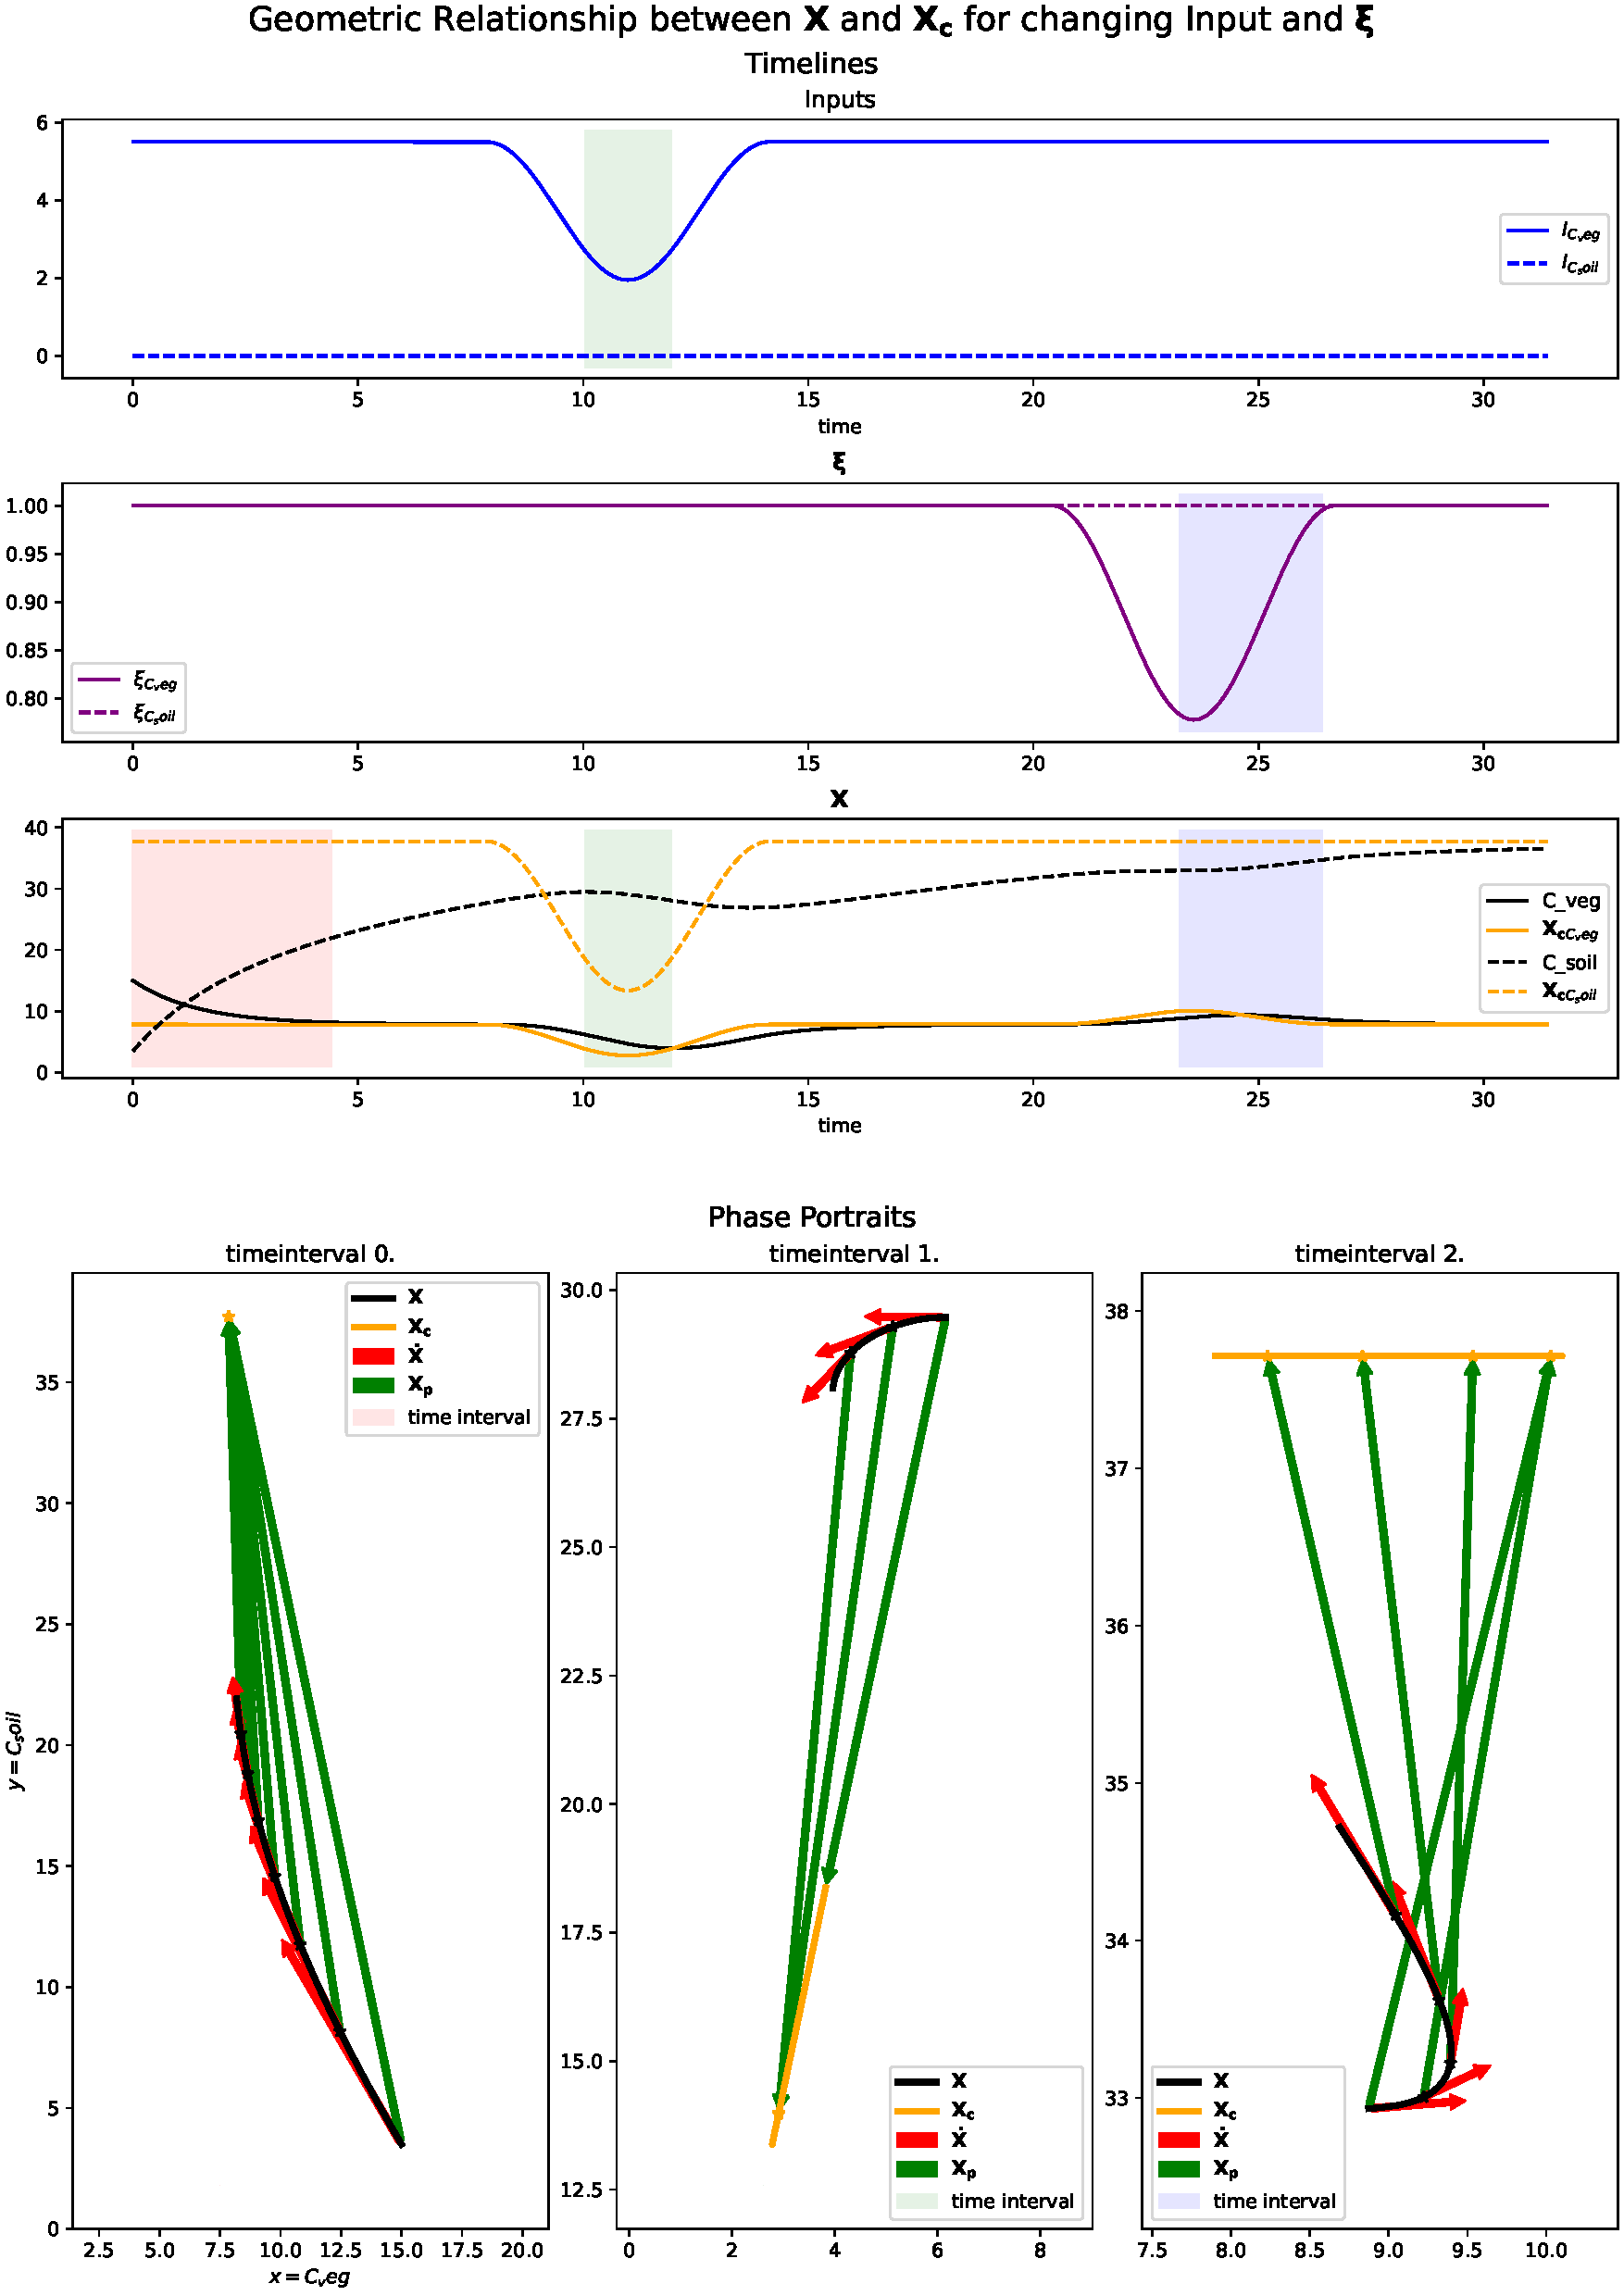
\includegraphics[height=.9\textheight]{figures/combined_timelines_and_2d_phase_space.pdf}
\caption{
  \label{Xc2D}
}
\end{figure}

\begin{figure}[t]
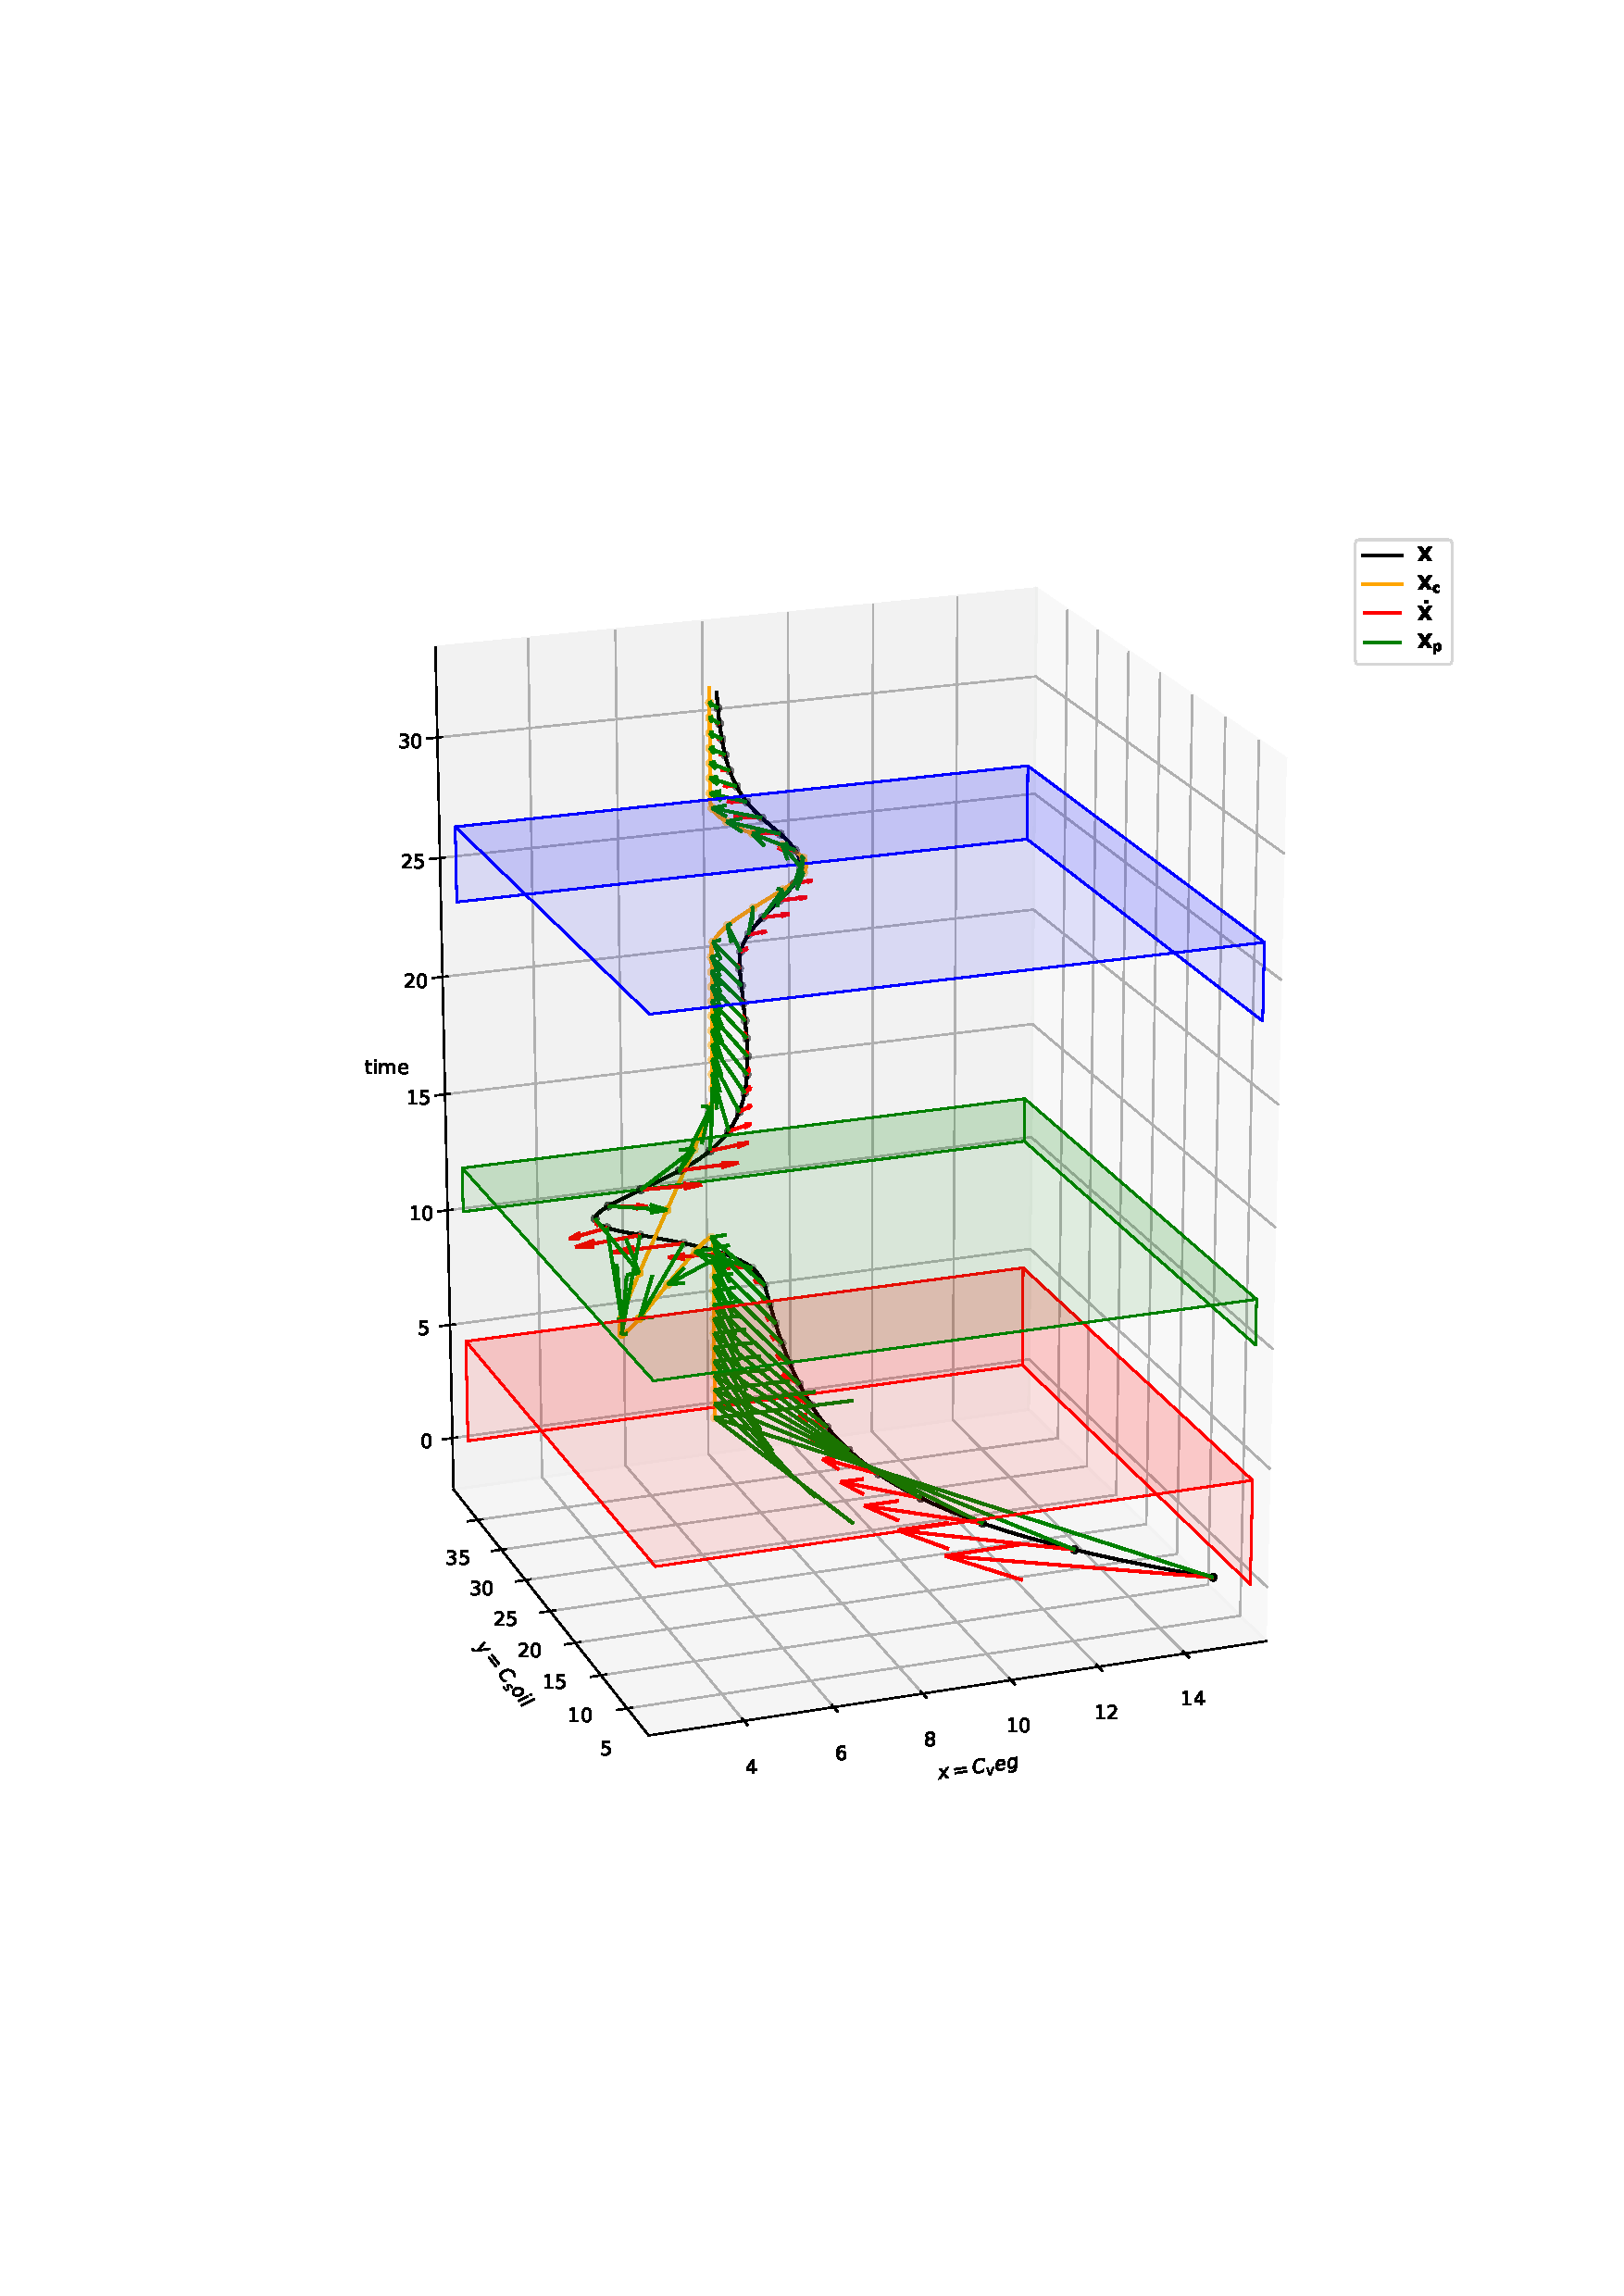
\includegraphics[height=.9\textheight]{figures/plot_vector_3d_X_Xc_time_z.pdf}
\caption{
  \label{Xc3D}
  %The 3D plot shows the same trajectories as \figref{}
  %For the first period
  %of its timeline (bottom) to $t\approx 2\pi$. In this period $X_c$ stays constant and
  %$X$ gradually approaches $X_c$ (although the derivative is not parallel to $X_p$).
  %after}
}
\end{figure}
\subsubsection{surrogate system for the overall mass}
We are aming at something like this:
$$
\dot{x}=u(t)-m(t)x
$$ 
where $x$ is the aggregated mass over all pools.
The question is how to specify $m(t)$ to insure this.

We start with the special case of a linear but nonautonoumous system (which is the subject of \citep{Luo2017Biogeosciences}):
$$
\frac{d \X}{d t}= \I(t) - M(t) \X 
$$
Taking the sum over all pools yields.
$$
\sum_{p \in pools} \left( \frac{d \X}{d t} \right)_p
=
\left( \I(t) - M(t) \X \right)_p
$$

With: 
$$
u=\sum_{p \in pools} (\I)_p, 
$$
$$
x = \sum_{p \in pools} (\X)_p
\text{ and }
$$ 
$$
\sum_{p \in pools} \left( \frac{d \X}{d t} \right)_p
=\frac{d}{d t}\sum_{p \in pools} (\X )_p
=\frac{d}{d t} x
$$
We can now try to costruct our new system for the combined mass $x$, in particular we want to find a function for the time dependent rate $m(t)$ such that. 
$$
\dot{x}
=u(t)-m(t) x 
=\sum_{p \in pools} \left( \I(t) - M(t) \X \right)_p
=u(t)-\sum_{p \in pools} ( M(t) \X )_p
$$
This yields: 
$$
m(t) = \frac{
    \sum_{p \in pools} ( M(t) \X )_p
    }{
    \sum_{p \in pools} (\X)_p
    }
$$
Notes:
\begin{enumerate}
\item 
  $m$ will in general be a function of time $m(t)$ even if the original matrix $M$ is not.
  This becomes apparrent when we consider that we need the vector $\X$ for every $t$ to define $m(t)$, which means that we also must solve the original system at least simultaneously.
  Assuming that we have done so \emph{before} we we can write a little more obviously.
  $$
  m(t) = \frac{
      \sum_{p \in pools} ( M \X(t) )_p
      }{
      \sum_{p \in pools} (\X(t))_p
      }
  $$
  Intuitively this reflects that the original system can have different rates for different pools and so the overall 
  rate depends on how mass is distributed between the pools initially and by the input streams. 
  The fact that the surrogate system is specific to a particular solution of the original system becomes even more apparent
  if we build surrogate systems for a nonlinear system. 
\item
  Consider a nonlinear systems
  $$
  \frac{d \X}{d t}= \I(\X,t) - M(\X,t) \X 
  $$
  Assume that we first solve the system numerically and therefore have $\X(t)$ available.
  Substituting the solution we get a linear system:
  $$
  \frac{d \X}{d t}= \tilde{\I}(t) - \tilde{M}(t) \X 
  $$
  with 
  $$
  \tilde{\I}(t)=\I(\X(t),t)
  $$
  and
  $$
  \tilde{M}(t)=M(\X(t),t)
  $$
  Which allows us to construct a one pool surrogate system with the same solution.
\end{enumerate}

The connection between the directions of $X_c$ and $X$ can be formalized in the following observations.

\begin{observation}[$x_p$ and $\dot{x}$ for the surrogate system]
With
\begin{align*}
\dot{x}   &=   u(t)-m(t)x              \\
x_c       &=   \frac{1}{m(t)} u(t)    \\
x_p       &=   x_c-x                  \\
          &=   \frac{1}{m(t)} \dot{x} 
\end{align*}
we have:
\begin{align}
\label{sign}
\sign \dot{x} &= \sign x_p
\end{align}
Which means that the solution $x$ always increases if $x<x_c$ and always decreases if $x>x_c$.
This is clear since $m(t) \ge 0 \quad \forall t$ (in compartmental systems only positive fluxes are allowed) and $m \ne 0$ for $x_p$ and $x_c=\frac{1}{m(t)} u$ to be defined.
\end{observation}

\begin{observation}[$\X_p$ and $\dot{\X}$ are not parallel]
An attempt to generalize \eqref{sign} to vectors in the sense that $\X_p$ and $\dot{\X}$ point in the same direction fails.
In \figref{Xc3D} the temporal evolution of $\X_c$ and $\X$ for an example two pool system is plotted,
which shows that in general $\X_p$ and $\dot{\X}$ are not pointing in the same direction.
\begin{align}
\frac{d}{dt}\left[\begin{matrix}C_{veg}\\C_{soil}\end{matrix}\right] = \left[\begin{matrix}I_{veg}{\left(t \right)}\\0\end{matrix}\right] + \left[\begin{matrix}- \left(r_{veg2out} + r_{veg2soil 0}\right) \xi_{veg}{\left(t \right)} & 0\\r_{veg2soil 0} \xi_{veg}{\left(t \right)} & - r_{soil2out}\end{matrix}\right] \left[\begin{matrix}C_{veg}\\C_{soil}\end{matrix}\right]
\end{align}
\begin{align}
\left[\begin{matrix}\frac{1}{\left(r_{veg2out} + r_{veg2soil 0}\right) \xi_{veg}{\left(t \right)}} & 0\\\frac{r_{veg2soil 0}}{r_{soil2out} \left(r_{veg2out} + r_{veg2soil 0}\right)} & \frac{1}{r_{soil2out}}\end{matrix}\right]
\end{align}
\begin{align}
\left[\begin{matrix}\frac{I_{veg}{\left(t \right)}}{\left(r_{veg2out} + r_{veg2soil 0}\right) \xi_{veg}{\left(t \right)}}\\\frac{r_{veg2soil 0} I_{veg}{\left(t \right)}}{r_{soil2out} \left(r_{veg2out} + r_{veg2soil 0}\right)}\end{matrix}\right]
\end{align}
This is even the case if we only consider autonomous systems.
Although $\X_c$ IS the unique stable fixpoint (and therefore an attractor) for $\tilde{\X}$ the  solution of the autonomous system, even $\dot{\tilde{\X}}$ does in general NOT point in the direction of $\X_c-\tilde{\X}$. This is a reflection of the internal pool structure as represented in  $M$. Compartmental systems are in general not obliged to move straight through phase space.   
%E.g. a serial system of three pools can only get material from pool 1 to pool 3 via pool 2. This might dictate a curved path to the equilibrium value, temporarily increasing the content of the
%intermediate pool.
\end{observation}

\begin{observation}[Direction of $\X_p$ and $\dot{\X}$]
A minimal attempt to generalize \eqref{sign} is the following:
If $M(t)$ is invertable 
% (this excludes zero rates) 
and if all components of the derivative $\dot{\X}$ have the same sign then all components of the $\X_p=\X_c-\X$ have the same sign too.
In other words if $\dot{\X}$ occupies the non negative orthant so does $\X_p$ and if $\dot{\X}$ occupies the non positive orphant so does $\X_p$. In both cases the scalar product $\langle \dot{\X},\X_p \rangle \ge 0$

Proof:
Using that $M(t)$ is invertable we can write the steady state solution $\X^*$ (for the system frozen at time $t$) for a given constant input $\I$ and Matrix $M$ as
\begin{align}
\X^*=M^{-1}\I
\end{align}
We first convince ourselfes that the matrix $M^{-1}$ has indeed only positive elements.
For a compartmental system the pool contents and imputs are alway positive.
This is also true for the steady state values of the frozen system.
If we choose $\I = (1,0,\dots, 0) $ we get $\X^*=M_{:,1}$ so we know that 
the first column of $M$ must be positive. 
We can do this with any column to obtain $M_{i,j}>0 \quad \forall i,j$.
If we assume further that the derivative $\dot{\X}$ has only positive components then the components of 
$\X_p$ are sums of products of positive values and have to be positive too.
In case all the components of $\dot{\X}$ are negative then the components of $\X_p$ are negative by the same arguement.
A consequence of this statement is that in case $\dot{\X}$ is either completely in the positive or negative orthant the inner product $\langle \dot{\X},\X_p \rangle \ge 0$ which means that the angle between them is smaller than a right angle.

Unfortunately this argument only applies to the very special cases that all pools increase or decrease simultaneously.
In general $\dot{\X}$ as well as $\X_p$ can have positive and negative components but in this case the knowledge of the positivity
of $M^{-1}$ is not sufficient to confine the difference in their directions.
\end{observation}

\begin{observation}[Direction of $\X_p$ and $\dot{X}$ in special cases]
The previous observation leads to the conjecture that perhaps $\langle \dot{\X},\X_p \rangle \ge 0$ is generally true, even if $M_{i,j} > 0 $ is not sufficient to prove it.
There are however special cases where this can be acertained.
If we talk about $\X_c$ at all we assume the existence of a stable fixedpoint for the frozen system. A necessarry (and sufficient) condition for this is that the real parts of all the eigenvalues of $M$ are greater than zero. 
In case all the eigenvalues are real we can express $\X_p$ and $\dot{\X}$ and the linear mapping encoded by $M$ in terms of tbe eigenvectors $e_1,\dots e_n$ and eigenvalues $\lambda_1, \dots \lambda_n$.
\begin{align}
\langle \dot{\X},\X_p  \rangle 
&=
\langle M \X_p,\X_p  \rangle \\
&=
\langle 
  \lambda_1 e_1 {x_p}_1+\dots \lambda_n e_n {x_p}_n , 
  e_1 {x_p}_1+\dots e_n {x_p}_n
\rangle 
\\
&=
\lambda_1 {x_p}_1^2 \langle e_1,e_1 \rangle
+\dots +
\lambda_n{x_p}_n^2 \langle e_n,e_n \rangle
\\
&> 0.
\end{align}
A noteworthy application are two dimensional compartmental linear systems with constant $M$ which can not have complex eigenvalues (Since the complex eigenvalues of real matrices always come in conjugate pairs the matrix of a two dimensional system would describe a rotation with shrinking radius (negative real part). For $\X$ on one of the boundaries of the positive orthant this would lead to a derivative pointing outwards and thus to negative pool contents, violating the assumption of a compartmental system).
If the system has more than two dimensions complex eigenvalues become possible and the discussion more complicated.
\end{observation}


\conclusions  %% \conclusions[modified heading if necessary]
TEXT
{\color{red} summary still missing}

\begin{enumerate}
\item
$X_c$ is not an attractor for $\X$ neither is $x_c$ for $x$ (overall mass)
All derived variables like $\RT$ and $\tau$ have to be interpreted in the context of the 'frozen' systems \emph{in equilibrium}.
\item
$\bar{X_c}$ as proxy for $\X$ depends on the time interval (examples show minimal error of about 7/100)
\item
$\xi$ is not a model property but a property of the literature
In attributions it is saver to look at $k \xi$ 


\end{enumerate}

%% The following commands are for the statements about the availability of data sets and/or software code corresponding to the manuscript.
%% It is strongly recommended to make use of these sections in case data sets and/or software code have been part of your research the article is based on.

\codeavailability{TEXT} %% use this section when having only software code available


\dataavailability{TEXT} %% use this section when having only data sets available


\codedataavailability{TEXT} %% use this section when having data sets and software code available


\sampleavailability{TEXT} %% use this section when having geoscientific samples available


\videosupplement{TEXT} %% use this section when having video supplements available


\appendix
\section{$\xi$}    %% Appendix A

\subsection{Examples where the actual value of $\xi$ matters or does not matter}     %% Appendix A1, A2, etc.
\label{xi_examples}
E.g. consider variance attribution via covariance as described in the supplementary materia S(9) of \citep{Zhou2018JOC}.
The relative contribution $RVar(a b)_a$ of variable $a$ to the variance of the product $a b$ is defined as 
\begin{align}
  \label{covln}
  RVar(a b)_a = \frac{cov(ln(a),ln(a b)}{Var(ln(a b)} 
\end{align}
As an example for an attribution that is independent of the arbitrary $d$
consider the question of temporal variance of $rt$ to it's factors $\xi$ and
$br$ via (tenporal) covariance of $rt$ with $\xi$ and $k$ since the temporal
covariance $ cov(ln(k),ln(rt))=0 $ but it is also obvious that an attribution to
the temporal change of $\xi$ leads to the same result as an attribution to the
product $\xi k$, so the distinction between contributions of $\xi$ and $k$ is
not necessary.  
% {\color{blue} perhaps cite \citep{Jiang2017James} if I find the
% place where the attribution is described. Actually the total difference in
% $\xi(t_{end})-\xi(t_0)$ is discussed which \emph{would} change with a scaled $\xi$
% but this does not seem to matter in the paper (since it is the same model and
% the \emph{same} $k$ and $\xi$ are used } 
An example where the result does
depend on the arbitrary $d$ is given by the attribution of the variance of $\RT$
of model ensemble to the variance of $\xi$ and $k$ via the same method as the
following minimal ensemble of two models shows. If we look at the contribution
of $\xi$ to the variance
\begin{align}
{var_{\xi}}_{rel} = \frac{
  cov([ln(\xi_1),ln(\xi_2)]^T,[ln(\frac{k_1}{\xi_1}),ln(\frac{k_2}{\xi_2})]^T)
}{
  var([ln(\frac{k_1}{\xi_1}),ln(\frac{k_2}{\xi_2})]^T)
}
\end{align}
If we rewrite the second model in the vector wiht an arbitrary $d$ we get a different result



\noappendix       %% use this to mark the end of the appendix section. Otherwise the figures might be numbered incorrectly (e.g. 10 instead of 1).

%% Regarding figures and tables in appendices, the following two options are possible depending on your general handling of figures and tables in the manuscript environment:

%% Option 1: If you sorted all figures and tables into the sections of the text, please also sort the appendix figures and appendix tables into the respective appendix sections.
%% They will be correctly named automatically.

%% Option 2: If you put all figures after the reference list, please insert appendix tables and figures after the normal tables and figures.
%% To rename them correctly to A1, A2, etc., please add the following commands in front of them:

\appendixfigures  %% needs to be added in front of appendix figures

\appendixtables   %% needs to be added in front of appendix tables

%% Please add \clearpage between each table and/or figure. Further guidelines on figures and tables can be found below.



\authorcontribution{TEXT} %% this section is mandatory

\competinginterests{TEXT} %% this section is mandatory even if you declare that no competing interests are present

\disclaimer{TEXT} %% optional section

\begin{acknowledgements}
TEXT
\end{acknowledgements}




%% REFERENCES

%% The reference list is compiled as follows:

%%\begin{thebibliography}{}
%%
%%\bibitem[AUTHOR(YEAR)]{LABEL1}
%%REFERENCE 1
%%
%%\bibitem[AUTHOR(YEAR)]{LABEL2}
%%REFERENCE 2
%%
%%\end{thebibliography}

%% Since the Copernicus LaTeX package includes the BibTeX style file copernicus.bst,
%% authors experienced with BibTeX only have to include the following two lines:
%%
%% \bibliographystyle{copernicus}
%% \bibliography{example.bib}
%%
%% URLs and DOIs can be entered in your BibTeX file as:
%%
%% URL = {http://www.xyz.org/~jones/idx_g.htm}
%% DOI = {10.5194/xyz}


%% LITERATURE CITATIONS
%%
%% command                        & example result
%% \citet{jones90}|               & Jones et al. (1990)
%% \citep{jones90}|               & (Jones et al., 1990)
%% \citep{jones90,jones93}|       & (Jones et al., 1990, 1993)
%% \citep[p.~32]{jones90}|        & (Jones et al., 1990, p.~32)
%% \citep[e.g.,][]{jones90}|      & (e.g., Jones et al., 1990)
%% \citep[e.g.,][p.~32]{jones90}| & (e.g., Jones et al., 1990, p.~32)
%% \citeauthor{jones90}|          & Jones et al.
%% \citeyear{jones90}|            & 1990

\bibliographystyle{copernicus}
\bibliography{TEE-clean.bib}


%% FIGURES

%% When figures and tables are placed at the end of the MS (article in one-column style), please add \clearpage
%% between bibliography and first table and/or figure as well as between each table and/or figure.

% The figure files should be labelled correctly with Arabic numerals (e.g. fig01.jpg, fig02.png).


%% ONE-COLUMN FIGURES

%%f
%\begin{figure}[t]
%\includegraphics[width=8.3cm]{FILE NAME}
%\caption{TEXT}
%\end{figure}
%
%%% TWO-COLUMN FIGURES
%
%%f
%\begin{figure*}[t]
%\includegraphics[width=12cm]{FILE NAME}
%\caption{TEXT}
%\end{figure*}
%
%
%%% TABLES
%%%
%%% The different columns must be seperated with a & command and should
%%% end with \\ to identify the column brake.
%
%%% ONE-COLUMN TABLE
%
%%t
%\begin{table}[t]
%\caption{TEXT}
%\begin{tabular}{column = lcr}
%\tophline
%
%\middlehline
%
%\bottomhline
%\end{tabular}
%\belowtable{} % Table Footnotes
%\end{table}
%
%%% TWO-COLUMN TABLE
%
%%t
%\begin{table*}[t]
%\caption{TEXT}
%\begin{tabular}{column = lcr}
%\tophline
%
%\middlehline
%
%\bottomhline
%\end{tabular}
%\belowtable{} % Table Footnotes
%\end{table*}
%
%%% LANDSCAPE TABLE
%
%%t
%\begin{sidewaystable*}[t]
%\caption{TEXT}
%\begin{tabular}{column = lcr}
%\tophline
%
%\middlehline
%
%\bottomhline
%\end{tabular}
%\belowtable{} % Table Footnotes
%\end{sidewaystable*}
%
%
%%% MATHEMATICAL EXPRESSIONS
%
%%% All papers typeset by Copernicus Publications follow the math typesetting regulations
%%% given by the IUPAC Green Book (IUPAC: Quantities, Units and Symbols in Physical Chemistry,
%%% 2nd Edn., Blackwell Science, available at: http://old.iupac.org/publications/books/gbook/green_book_2ed.pdf, 1993).
%%%
%%% Physical quantities/variables are typeset in italic font (t for time, T for Temperature)
%%% Indices which are not defined are typeset in italic font (x, y, z, a, b, c)
%%% Items/objects which are defined are typeset in roman font (Car A, Car B)
%%% Descriptions/specifications which are defined by itself are typeset in roman font (abs, rel, ref, tot, net, ice)
%%% Abbreviations from 2 letters are typeset in roman font (RH, LAI)
%%% Vectors are identified in bold italic font using \vec{x}
%%% Matrices are identified in bold roman font
%%% Multiplication signs are typeset using the LaTeX commands \times (for vector products, grids, and exponential notations) or \cdot
%%% The character * should not be applied as mutliplication sign
%
%
%%% EQUATIONS
%
%%% Single-row equation
%
%\begin{equation}
%
%\end{equation}
%
%%% Multiline equation
%
%\begin{align}
%& 3 + 5 = 8\\
%& 3 + 5 = 8\\
%& 3 + 5 = 8
%\end{align}
%
%
%%% MATRICES
%
%\begin{matrix}
%x & y & z\\
%x & y & z\\
%x & y & z\\
%\end{matrix}
%
%
%%% ALGORITHM
%
%\begin{algorithm}
%\caption{...}
%\label{a1}
%\begin{algorithmic}
%...
%\end{algorithmic}
%\end{algorithm}
%
%
%%% CHEMICAL FORMULAS AND REACTIONS
%
%%% For formulas embedded in the text, please use \chem{}
%
%%% The reaction environment creates labels including the letter R, i.e. (R1), (R2), etc.
%
%\begin{reaction}
%%% \rightarrow should be used for normal (one-way) chemical reactions
%%% \rightleftharpoons should be used for equilibria
%%% \leftrightarrow should be used for resonance structures
%\end{reaction}
%
%
%%% PHYSICAL UNITS
%%%
%%% Please use \unit{} and apply the exponential notation
\section{to do}
\begin{enumerate}
\item
  finish the figure
\item
  \sout{introduce the 1D surrogate systems}
\item
  \sout{Prove the geometric Observations} 
\item
  Put the definition for attractors in the text
\item 
To explain the 1 pools system tendency to "chase" $X_c$ we can rephrase it the other way around to:
At a given point $t_f$the derivative is determined by the present $m_f=m(t_f)$ 
and the present input $i_f=i(t_f)$:$\dot{x} = i_f-m_f x_f$ 
The derivative at this point determines the possible equilibrium of the frozen linear system with the same derivative at this point.
If the derivative is positive we have 
\begin{align*}
0 < if - m_f x \\
\rightarrow 
m_f x & < i_f \\
\rightarrow 
x < \frac{1}{m_f} i_f=x_f* = x_c
\end{align*}
So the prospectimve equilibrium of the frozen system is bigger than the current value.
\end{enumerate}
\end{document}
